\documentclass{article}
\usepackage{
  fancyhdr,
  amsmath,
  amsfonts,
  bm,
  pgfplots,
  float,
  multicol,
  cancel,
}
\usepackage[inline]{enumitem}

% Don't indent paragraphs
\setlength\parindent{0pt}

% meta data
\newcommand{\authorname}{Amo DelBello}
\newcommand{\classname}{Calculus I, Math 1510}
\newcommand{\assignment}{Assignment \#1}

% headers
\newcommand{\problem}[2]{\vspace{5ex}\section*{Section #1, Problem #2}}
\newcommand{\solution}{\subsection*{Solution}}

\title{\classname\ | \assignment}
\author{\authorname}
\date{\today}

% Default plot style
\pgfplotsset{
    DefaultPlotStyle/.style={
      small,
      axis lines = center,
      xlabel = $x$,
      ylabel = {$f(x)$},
      xlabel style={below right},
      ylabel style={above left},
      grid=both,
      grid style={line width=.1pt, draw=gray!10},
      major grid style={line width=.2pt,draw=gray!50},
      % axis lines=middle,
      % minor tick num=5,
    },
  }

\fancyhf{}
\pagestyle{fancy}
\fancyhead[LO,LE]{\authorname}
\fancyhead[CO,CE]{\classname}
\fancyhead[RO,RE]{\assignment}
\pgfplotsset{width=10cm,compat=1.9}
\setlength\columnsep{20pt}

% TODO: The bold beginnings of some questions
\begin{document}
\maketitle

%%%%%%%%%%%%%%%%%%%%%%%%%%%%%%%%%%%%
% Problem 1.1 7
%%%%%%%%%%%%%%%%%%%%%%%%%%%%%%%%%%%%
\problem{1.1}{7}
Determine the domain and range of $ g(x) = 3x^2 - 10 $.

\solution\
\begin{description}
  \item[Domain:] $g$ is defined for all values of $x$. Its domain is the set of all real numbers, written:
    \[
      D = (-\infty, \infty) \quad \text{or} \quad \mathbb{R}
    \]
  \item[Range:] Because $x^2 \geq 0$ for all $x$, it follows that $3x^2 - 10 \geq 10$, which implies
    that the range of $f$ is:
    \[
      R = [-10, \infty]
    \]
\end{description}

%%%%%%%%%%%%%%%%%%%%%%%%%%%%%%%%%%%%
% Problem 1.1 9
%%%%%%%%%%%%%%%%%%%%%%%%%%%%%%%%%%%%
\problem{1.1}{9}
\textbf{Water tower} A cylindrical water tower with a radius of 10 m and a height
of 50 m is filled to a height of $h$ m. The volume $V$ of water (in cubic meters) is given by the
function $g(h) = 100\pi h$. Identify the independent and dependent variables for this function, and then
determine an appropriate domain.

\solution\
\begin{description}
\item[Independent variable:] The independent variable is the variable associated with the domain.
  Therefore in $100\pi h$ the independent variable is $h$.
\item[Dependent variable:] The dependent variable is the variable associated with the range. In
  $V = g(h)$ the dependent variable is $V$.
\item[Appropriate domain:] As the height of the water tower is 50 m, the domain is $0$ (when the
  tower is empty) to $50$ (when the tower is full):
  \[
    D = 0 \leq h \leq 50
  \]
\end{description}

%%%%%%%%%%%%%%%%%%%%%%%%%%%%%%%%%%%%
% Problem 1.1 23
%%%%%%%%%%%%%%%%%%%%%%%%%%%%%%%%%%%%
\problem{1.1}{23}
State the domain and range of the function
\[
  f(x) = \frac{x^2 - 5x + 6}{x - 2}
\]

\solution\
\begin{description}
\item[Domain:] The domain of the function is all real numbers that don't cause the denominator of the expression to evaluate to $0$. Therefore the domain of the function is:
  \[
    D = \{x: x \neq 2\}
  \]
\item[Range:]
  \begin{multicols}{2}
    The range of the function is all real numbers except the number $-1$ because $y$ is undefined at
    $x = 2$ and that's where it \textit{would} be $-1$.
    \[
      R = \{y: y \neq -1\}
    \]
  \columnbreak\
    \begin{figure}[H]
      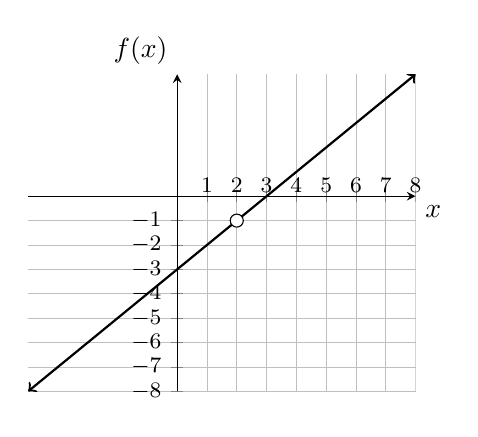
\begin{tikzpicture}
        \begin{axis}[
          DefaultPlotStyle,
          x tick label style={above},
          xtick={0,1,...,8},
          ytick={-10,-9,...,0},
        ]

          % Plot the function
          \addplot[
            domain=-5:8,
            thick,
            <->,
          ]
          { (x^2 - (5 * x) + 6) / (x - 2) };

          % Where `x` is not defined
          \node[
            circle,
            fill=white,
            draw=black,
            scale=0.5,
          ]
          at (axis cs:2,-1){};
        \end{axis}
      \end{tikzpicture}
    \end{figure}
  \end{multicols}
\end{description}

%%%%%%%%%%%%%%%%%%%%%%%%%%%%%%%%%%%%
% Problem 1.1 27
%%%%%%%%%%%%%%%%%%%%%%%%%%%%%%%%%%%%
\problem{1.1}{27}
State the domain of the function
\[
  h(u) = \sqrt[3]{u - 1}
\]

\solution\
As a cubed root is an odd numbered root, the result when evaluated will always equal a real number. Therefore the domain of the function is all real numbers:
\[
  D = (-\infty, \infty) \quad \text{or} \quad \mathbb{R}
\]

%%%%%%%%%%%%%%%%%%%%%%%%%%%%%%%%%%%%
% Problem 1.1 31
%%%%%%%%%%%%%%%%%%%%%%%%%%%%%%%%%%%%
\problem{1.1}{31}
\textbf{Launching a rocket} A small rocket is launched vertically upward from the
edge of a cliff 80 ft above the ground at a speed of 96 ft/s. Its height (in feet) above the ground
is given by $h(t) = -16t^2 + 96t + 80$, where $t$ represents time measured in seconds.

\begin{enumerate}[label=\textbf{\alph*. }]
\item Assuming the rocket is launched at $t = 0$, what is an appropriate domain for $h$?
\item Graph $h$ and determine the time at which the rocket reaches its highest point. What is the
  height at that time
\end{enumerate}

\solution\
\begin{enumerate}[label=\textbf{\alph*. }]
\item
  We can find the domain of the function by using the quadratic equation
  \[
    \begin{split}
      x &= \frac{-96 \mp \sqrt{96^2 - 4(-16)(80)}}{2(-16)} \\
      x &= \frac{-96 \mp 119.733}{-32} \\
      x &= -.7416, \quad x = 6.742
    \end{split}
  \]
  Since the rocket is launched at $t=0$, the appropriate domain is
  \[
    \{x: 0 \leq x \leq 6.742 \}
  \]
\pagebreak
\item
\begin{multicols}{2}
  We can calculate the maximum of a parabola using $x = \dfrac{-b}{2a}$.
  \[
    \frac{-96}{2(-16)} = 3
  \]
  When we evaluate $h(3)$ we get
  \[
  \begin{split}
    y &= -16{(3)}^2 + 96(3) + 80 \\
    y &= -144 + 288 + 80 \\
    y &= 224
  \end{split}
  \]
\columnbreak\
\begin{figure}[H]
  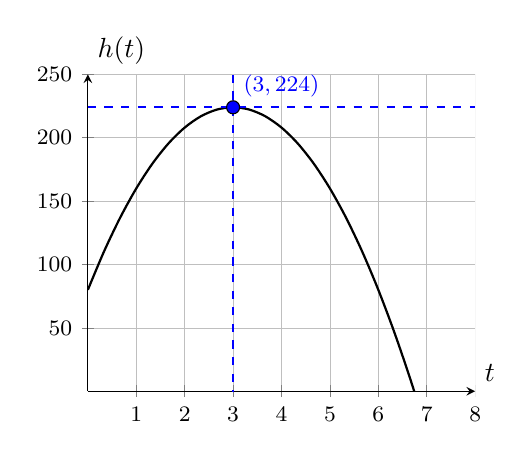
\begin{tikzpicture}
    \begin{axis}[
      DefaultPlotStyle,
      xlabel = $t$,
      ylabel = {$h(t)$},
      xlabel style={above right},
      ylabel style={above right},
      xtick={0,1,...,8},
      ytick={0,50,...,300},
      ymin=0,
      ymax=250,
      xmax=8
    ]

      % Plot the function
      \addplot[
        domain=0:8,
        range=0:200,
        smooth,
        thick,
        % <->,
      ]
      { -16*x^2 + 96* x + 80 };

      % domain at the highest point
      \draw[
      dashed,
      thick,
      blue,
      % <->
      ]
      (300,0)--(300,500);


      % range at the highest point
      \draw[
      dashed,
      thick,
      blue,
      % <->
      ]
      (0,400)--(800,400)
      node[above, xshift = -7em]
      {\footnotesize $(3, 224)$};

      % Where `x` is not defined
      \node[
        circle,
        fill=blue,
        draw=black,
        scale=0.5,
      ]
      at (axis cs:3,224){};
    \end{axis}
  \end{tikzpicture}
\end{figure}
\end{multicols}
\end{enumerate}

%%%%%%%%%%%%%%%%%%%%%%%%%%%%%%%%%%%%
% Problem 1.1 33 & 34
%%%%%%%%%%%%%%%%%%%%%%%%%%%%%%%%%%%%
\problem{1.1}{33 \& 34}
Let $f(x) = x^2 - 4$, $g(x) = x^3$, and $F(x) = 1/(x - 3)$. Simplify or evaluate the following
expressions.

\begin{enumerate}[label=\textbf{\arabic*. }]
  \setcounter{enumi}{32}
\item $g(1/z)$
  \solution\
  \[
    \begin{split}
      y &= {(1/z)}^3 \\
      y &= 1/z^3
    \end{split}
  \]

\item $F(y^4)$
  \solution\
  \[
    1/y^4 - 3
  \]
\end{enumerate}

%%%%%%%%%%%%%%%%%%%%%%%%%%%%%%%%%%%%
% Problem 1.1 47 & 48
%%%%%%%%%%%%%%%%%%%%%%%%%%%%%%%%%%%%
\problem{1.1}{47 \& 48}
Let $f(x) = |x|$, $g(x) = x^2 - 4$, $F(x) = \sqrt{x}$, and $G(x) = 1/(x - 2)$. Determine the
following composite functions and give their domains.

\begin{enumerate}[label=\textbf{\arabic*. }]
  \setcounter{enumi}{46}
\item $f \circ g$
  \solution\
  \[
    \begin{split}
      y &= f(g(x)) \\
      y &= f(x^ - 4) \\
      y &= |x^2 - 4|, D = \text{all real numbers or } \mathbb{R}
    \end{split}
  \]

\item $g \circ f$
  \solution\
  \[
    \begin{split}
      y &= g(f(x)) \\
      y &= g(|x|) \\
      y &= |x^2 - 4|, D = \text{all real numbers or } \mathbb{R}
    \end{split}
  \]
  \end{enumerate}

%%%%%%%%%%%%%%%%%%%%%%%%%%%%%%%%%%%%
% Problem 1.1 57 & 58
%%%%%%%%%%%%%%%%%%%%%%%%%%%%%%%%%%%%
\problem{1.1}{57 \& 58}
Let $g(x) = x^2 + 3$. Find a function $f$ that produces the given composition.

\begin{enumerate}[label=\textbf{\arabic*. }]
  \setcounter{enumi}{56}
\item $(f \circ g)(x) = x^4 + 6x^2 + 9$
  \solution\

  $x^4 + 6x^2 + 9$ factors to $(x^2 + 3)(x^2 + 3)$ or ${(x^2 + 3)}^2$. In order to produce the
  desired result with an argument of $g(x) = x^2 + 3$, $f(x)$ should be:
  \[
    f(x) = x^2
  \]
\item $(f \circ g)(x) = x^4 + 6x^2 + 20$
  \solution
  This problem is very similar to the above \#57 if we rewrite the result of the composition as
  $x^4 + 6x^2 + 9 \bm{+ 11}$. We can factor in the same way as above and then just add $11$ to the result: $(x^2 + 3)(x^2 + 3) + 11$. So the resulting $f(x)$ is
  \[
    f(x) = x^2 + 11
  \]
  \end{enumerate}

%%%%%%%%%%%%%%%%%%%%%%%%%%%%%%%%%%%%
% Problem 1.1 65 & 66
%%%%%%%%%%%%%%%%%%%%%%%%%%%%%%%%%%%%
\problem{1.1}{65 \& 66}
Simplify the difference quotient $\dfrac{f(x+h) - f(x)}{h}$ for the following functions

\begin{enumerate}[label=\textbf{\arabic*. }]
  \setcounter{enumi}{64}
\item $f(x) = x^2$
  \solution{}
  First we note that $f(x + h) = {(x + h)}^2$ or $x^2 + 2hx + h2$. We can substitute this expression into the difference quotient and simplify:
  \begin{align*}
    \frac{f(x + h) - f(x)}{h} &= \frac{(x^2 + 2hx + h^2) - x^2}{h} \\
                              &= \frac{2hx + h^2}{h} \\
                              &= \frac{2hx}{h} + \frac{h^2}{h} \\
                              &= 2x + h
  \end{align*}
\item $f(x) = 2x^2 - 3x + 1$
  \solution{}
  First we note that $f(x + h) = 2{(2 + h2)}^2 - 3(x + h) + 1$. We can substitute this expression into the difference quotient and simplify:
  \begin{align*}
    \frac{f(x + h) - f(x)}{h} &= \frac{f(x + h) = 2{(2 + h2)}^2 - 3(x + h) + 1 - (2x^2 - 3x + 1)}{h} \\
                              &= \frac{2(x+h)(x+h) - 3x -3h + 1 - (2x^2 - 3x + 1)}{h} \\
                              &= \frac{2(x^2 + 2hx + h^2) - 3x - 3h + 1 - 2x^2 + 3x -1}{h} \\
                              &= \frac{\cancel{2x^2} + 4hx + 2h^2 - \cancel{3x} - 3h + \cancel{1} - \cancel{2x^2} + \cancel{3x} - \cancel{1}}{h} \\
                              &= \frac{4 \cancel{h} x + 2 \cancelto{h}{h^2} - 3 \cancel{h}}{\cancel{h}} \\
                              &= 4x + 2h - 3
  \end{align*}
\end{enumerate}

\pagebreak

%%%%%%%%%%%%%%%%%%%%%%%%%%%%%%%%%%%%
% Problem 1.2 1
%%%%%%%%%%%%%%%%%%%%%%%%%%%%%%%%%%%%
\problem{1.2}{1}
Give four ways in which functions may be defined and  represented.

\solution{}
\begin{enumerate}
  \item Formulas
  \item Graphs
  \item Tables
  \item Words
\end{enumerate}

%%%%%%%%%%%%%%%%%%%%%%%%%%%%%%%%%%%%
% Problem 1.2 3
%%%%%%%%%%%%%%%%%%%%%%%%%%%%%%%%%%%%
\problem{1.2}{3}
Determine the function $f$ represented by the graph of the line $y = f(x)$ in the figure.
(Given points are $(0, -1)$ \& $(3, -1)$)
% TODO: Plot graph from the question

\solution{}
From the point $(0, -1)$ we can determine that the $y$ intercept is $-1$. We can also determine the
slope using $m = \dfrac{y_2 - y2}{x_2 - x_1}$:
\[
  \frac{-3 - (-1)}{3 - 0} = -\frac{2}{3}
\]
Therefore the function $f$ is
\[
  f = -\frac{3}{2}x - 1
\]

%%%%%%%%%%%%%%%%%%%%%%%%%%%%%%%%%%%%
% Problem 1.2 23
%%%%%%%%%%%%%%%%%%%%%%%%%%%%%%%%%%%%
\problem{1.2}{23}
\textbf{Bald eagle population} After DDT was banned and the Endangered Species Act was passed in
1973, the number of bald eagles in the United States increased dramatically. In the lower 48 states,
the number of breeding pairs of bald eagles increased at a nearly linear rate from 1875 pairs in
1986 to 6471 pairs in 2000.

\begin{enumerate}[label=\textbf{\alph*. }]
  \item Use the data points for 1986 and 2000 to find a linear function p that models the number of
    breeding pairs from 1986 to 2000 $(0 \leq t \leq 14)$.
  \item Using the function in part (a), approximately how many breeding pairs were in the lower 48
    states in 1995?
\end{enumerate}

\solution{}
\begin{enumerate}[label=\textbf{\alph*. }]
\item
  As we are dealing with the domain $(0 \leq t \leq 1)4$, our starting year (1986) can be considered
  to be $t = 0$. So given the point for 1986 \-- $(0, 1875)$ we see that our $y$ intercept is
  $1875$. We can consider our second point from 2000 to be $(14, 6471)$. Using the formula for slope
  we can calculate our slope
  \[
    m = \frac{6471 - 1875}{14 - 0} = 328.285
  \]
  The linear function can then be expressed as
  \[
    y = 328.285x + 1875
  \]

\item
  Using our domain $(0 \leq t \leq 14)$, we can see that the year 1995 can be expressed as $9$.
  We can determine approximately how many breeding pairs were in 1995 by evaluating $f(9)$ using the
  formula above
  \begin{align*}
    f(9) &= 328.285(9) + 1875 \\
         &= 4829.565
  \end{align*}
\end{enumerate}

%%%%%%%%%%%%%%%%%%%%%%%%%%%%%%%%%%%%
% Problem 1.2 25 - 26
%%%%%%%%%%%%%%%%%%%%%%%%%%%%%%%%%%%%
\problem{1.2}{25 \-- 26}
\textbf{Defining piecewise functions} Write a definition of the function whose graph is given.

\begin{description}
  \item[25.]
  \solution{}
  We can see that $x = 3$ from $x \leq 3$ just by looking at the graph. For $x > 3$, we can determine
  the definition of the function by first calculating the slope using points from the graph, and then
  finding the $y$ intercept using substitution.

  \begin{description}
    \item[Slope:] Using the points $(4, 5)$ and $(5, 7)$ we can find the slope with
    \[
      \dfrac{7-7}{5-4} = 2
    \]
    \item[$y$ Intercept:] We can solve for the $y$ intercept using (4, 5):
      \begin{align*}
        2(4) + b &= 5 \\
               b &= 5 - 8 \\
                 &= -3
      \end{align*}
  \end{description}
  Now we can express the function definition for $x > 3$ as $2x -3$. So the whole piecewise function is
  \[
    f(x) = \begin{cases}
             -3   &\text{if } x \leq 3 \\
             2x-3 &\text{if } x > 3
           \end{cases}
  \]

  \item[26.]
  \solution{}
  There are two cases for this piecewise function: $(x < 3)$ and $(x \geq 3)$.
  \begin{description}
  \item[$x<3$:] We can see that the $y$ intercept is $1$ and we can calculate the slope using points
    ($(0,1)$ and $(3,4)$) on the graph: $\dfrac{4-1}{3-0} = 1$. The first case of the function can
    then be expressed as
    \[
      f(x) = x + 1
    \]

  \item[$x\geq3$:] Using substitution we can find the slope with the following points $(3,2), (6,1)$
    \[
      \dfrac{1-2}{6-3} = -\dfrac{1}{3}
    \]
    We can then determine the $y$ intercept by substituting the point $(3,2)$
    \begin{align*}
      f(3) = -\frac{1}{3}(3) + b &= 2 \\
                               b &= -1 -2 \\
                                 &= -3
    \end{align*}
    The second case of the function can then be expressed as
    \[
      f(x) = -\frac{1}{3} -3
    \]

  \end{description}
  We can then express the entire piecewise function like this
  \[
    f(x) = \begin{cases}
             x + 1 &\text{if } x < 3 \\
             -\frac{1}{3} - 3 &\text{if } x \geq 3
           \end{cases}
  \]
\end{description}

%%%%%%%%%%%%%%%%%%%%%%%%%%%%%%%%%%%%
% Problem 1.2 33 - 34
%%%%%%%%%%%%%%%%%%%%%%%%%%%%%%%%%%%%
\problem{1.2}{33 \-- 34}
\textbf{Piecewise linear functions} Graph the following functions.

\begin{description}
\item[33.]
  \[
    f(x) = \begin{cases}
             -2x - 1 &\text{if } x < -1 \\
             1 &\text{if } -1 \leq x \leq 1 \\
             2x - 1 &\text{if } x > 1
           \end{cases}
  \]
  \solution{}
  \begin{multicols}{2}
  I plotted some sensible $(x,y)$ coordinates using the functions provided.
  \begin{align*}
    x &= -4, \quad y = -2(-4)-1 = 7 \\
    x &= -2, \quad y = -2(-2)-1 = 3 \\
    x &= -1, \quad y = 1 \\
    x &= 1, \quad y = 1 \\
    x &= 2, \quad y = 4 - 1 = 3 \\
    x &= 4, \quad y = 8-1 = 7 \\
  \end{align*}

  \columnbreak\
  \begin{figure}[H]
      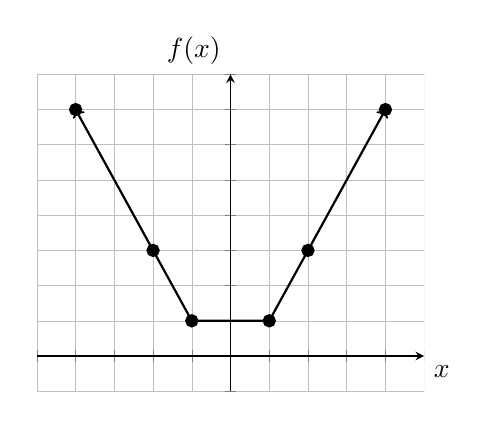
\begin{tikzpicture}
        \begin{axis}[
          DefaultPlotStyle,
          ymin = -1,
          ymax = 8,
          ytick={-1,0,...,8},
          yticklabels={,,},
          xmin = -5,
          xmax = 5,
          xtick={-5,-4,...,5},
          xticklabels={,,},
        ]

          \addplot[
            mark=*,
            mark size=2pt,
            thick,
            <->,
          ] plot coordinates
          { (-4, 7) (-2, 3) (-1, 1) (1, 1) (2, 3) (4, 7) };
        \end{axis}
      \end{tikzpicture}
    \end{figure}
  \end{multicols}

\item[34.]
  \[
    f(x) = \begin{cases}
             2x + 2 &\text{if } x < 0 \\
             x + 2 &\text{if } 0 \leq x \leq 2 \\
             3 - \frac{x}{2} &\text{if } x > 2
           \end{cases}
  \]
  \solution{}
  \begin{multicols}{2}
  I plotted some sensible $(x,y)$ coordinates using the functions provided.
  \begin{align*}
    x &= -3, \quad y = -2(-3)-2 = -4 \\
    x &= -1, \quad y = 0 \\
    x &= 0, \quad y = 2 \\
    x &= 2, \quad y = 4 \\
    x &= 3, \quad y = \frac{6}{2} - \frac{3}{2} = 1\frac{1}{2} \\
    x &= 5, \quad y = \frac{6}{2} - \frac{5}{2} = \frac{1}{2}
  \end{align*}

  \columnbreak\
  \begin{figure}[H]
      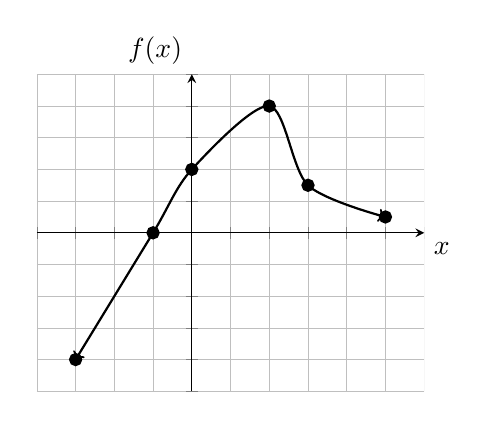
\begin{tikzpicture}
        \begin{axis}[
          DefaultPlotStyle,
          ymin = -5,
          ymax = 5,
          ytick={-5,-4,...,8},
          yticklabels={,,},
          xmin = -4,
          xmax = 6,
          xtick={-5,-4,...,6},
          xticklabels={,,},
        ]

          \addplot[
            mark=*,
            mark size=2pt,
            smooth,
            thick,
            <->,
          ] plot coordinates
          { (-3, -4) (-1, 0) (0, 2) (2, 4) (3, 1.5) (5, .5) };
        \end{axis}
      \end{tikzpicture}
    \end{figure}
  \end{multicols}

%%%%%%%%%%%%%%%%%%%%%%%%%%%%%%%%%%%%
% Problem 1.2 49 - 51
%%%%%%%%%%%%%%%%%%%%%%%%%%%%%%%%%%%%
\problem{1.2}{49 \-- 51}

  \textbf{Area functions} Let $A(x)$ be the area of the region bounded by the t-axis and the graph of
  $y = ƒ(t)$ from $t = 0$ to $t = x$. Consider the following functions and graphs.

  \begin{enumerate*}[label=\textbf{\alph*. }]
  \item Find $A(2) \,$
  \item Find $A(6) \,$
  \item Find a formula for $A(x)$
  \end{enumerate*}

  \begin{enumerate}[label=\textbf{\arabic*. }]
  \setcounter{enumi}{48}
    \item $f(t) = 6$
      \solution{}
      $A(x)$ is in the area bounded by the graph of $f$ and the t-axis from $t = 0$ to $t = x$.
      \begin{enumerate}[label=\textbf{\alph*. }]
        \item $A(2) = 2(6) = 12$
        \item $A(6) = 6(6) = 36$
        \item if $f(t) = 6$ then \\
            $A(x) = f(t) * x$ and \\
            $A(x) = 6$
      \end{enumerate}

    \item $f(t) = \dfrac{t}{2}$
      \solution{}
      We can use the formula for the area of a triangle
      \begin{enumerate}[label=\textbf{\alph*. }]
        \item $A(2) = \dfrac{1}{2}(2)\left(\dfrac{2}{2}\right) = 1$
        \item $A(6) = \dfrac{1}{2}(6)\left(\dfrac{6}{2}\right) = 9$
        \item
          \begin{flalign*}
            A(x) &= \frac{1}{2}x \left(\frac{x}{2}\right) &\\
                 &= \frac{1}{2} \left(\frac{x^2}{2}\right) &\\
                 &= \frac{x^2}{4}
          \end{flalign*}
      \end{enumerate}

    \item $f(t) = \begin{cases}
                    2t - 8   &\text{if } t \leq 3 \\
                    2 &\text{if } t > 3
                  \end{cases}$
                  \begin{enumerate}[label=\textbf{\alph*. }]
                  \item
                  \item
                  \item
                  \end{enumerate}
  \end{enumerate}

\end{description}

%%%%%%%%%%%%%%%%%%%%%%%%%%%%%%%%%%%%
% Problem 1.2 55
%%%%%%%%%%%%%%%%%%%%%%%%%%%%%%%%%%%%
\pagebreak
\problem{1.2}{55}
\textbf{Transformations of $f(x) = x^2$} Use shifts and scalings to transform the
graph of $ƒ(x) = x^2$ into the graph of $g$. Use a graphing utility to check your work.

\begin{enumerate}[label=\textbf{\alph*. }]
  \item
    \begin{multicols}{2}
      \begin{align*}
        g(x) &= f(x - 3) \\
             &= (x - 3)(x - 3) \\
             &= x^2 - 6x + 9
      \end{align*}
      \columnbreak\
        \begin{figure}[H]
          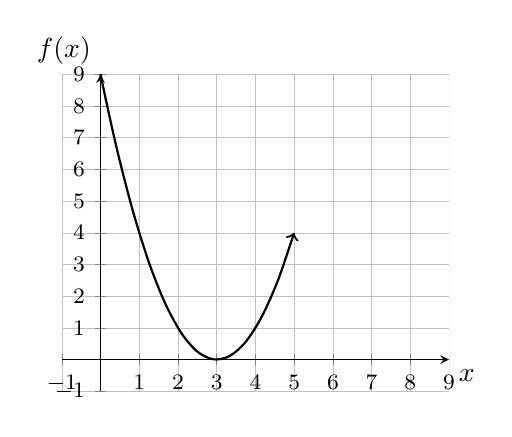
\begin{tikzpicture}
            \begin{axis}[
              DefaultPlotStyle,
              xmin = -1,
              xmax = 9,
              xtick={-1,-0,...,9},
              ymin = -1,
              ymax = 9,
              ytick={-1,0,...,9},
            ]

              \addplot[
                thick,
                smooth,
                <->,
              ]
              { x^2 - (6 * x) + 9 };
            \end{axis}
          \end{tikzpicture}
        \end{figure}
    \end{multicols}
  \item
    \begin{multicols}{2}
      \begin{align*}
        g(x) &= f(2x -4) \\
             &= (2x - 4)(2x - 4) \\
             &= 4x^2 - 8x + 16
      \end{align*}
      \columnbreak\
      \begin{figure}[H]
          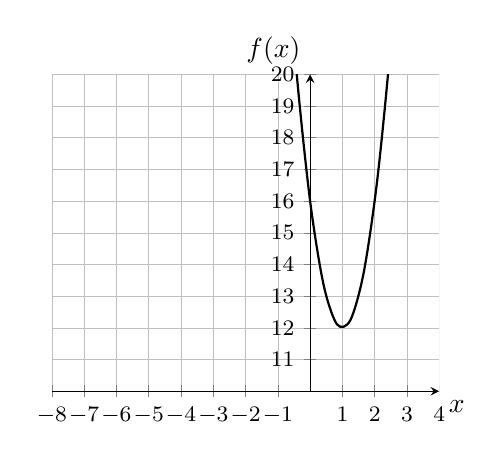
\begin{tikzpicture}
            \begin{axis}[
              DefaultPlotStyle,
              xmin = -8,
              xmax = 4,
              xtick={-8,-7,...,9},
              ymin = 10,
              ymax = 20,
              ytick={-10,-9,...,80},
            ]

              \addplot[
                thick,
                smooth,
                <->,
              ]
              { 4*x^2 - (8 * x) + 16 };
            \end{axis}
          \end{tikzpicture}
        \end{figure}
    \end{multicols}
  \item
    \begin{multicols}{2}
      \begin{align*}
        g(x) &= -3f(x - 2) + 4 \\
             &= -3(x - 2)(x -2) + 4 \\
             &= -3(x^2 - 4x + 4) + 4 \\
             &= -3x^2 + 12x - 4 + 4 \\
             &= -3x^2 + 12x
      \end{align*}
      \columnbreak\
      \begin{figure}[H]
          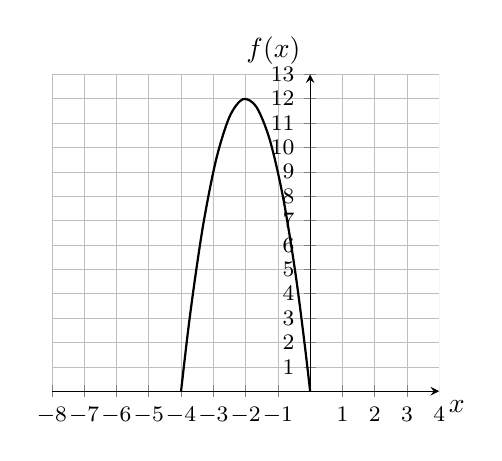
\begin{tikzpicture}
            \begin{axis}[
              DefaultPlotStyle,
              xmin = -8,
              xmax = 4,
              xtick={-8,-7,...,9},
              ymin = 0,
              ymax = 13,
              ytick={-10,-9,...,80},
            ]

              \addplot[
                thick,
                smooth,
                <->,
              ]
              { -3*x^2 - (12 * x) };
            \end{axis}
          \end{tikzpicture}
        \end{figure}
    \end{multicols}
  \item
    \begin{multicols}{2}
      \begin{align*}
        g(x) &= 6f\left(\frac{x-2}{3}\right) + 1 \\
             &= 6\left(\frac{x-2}{3}\right)\left(\frac{x-2}{3}\right) + 1 \\
             &= 6\left(\frac{x^2 - 4x + 4}{9}\right) + 1 \\
             &= \frac{6x^2 - 24x + 24}{9} + 1 \\
             &= \frac{2x^2 - 8x + 8}{3} + 1
      \end{align*}
      \columnbreak\
      \begin{figure}[H]
          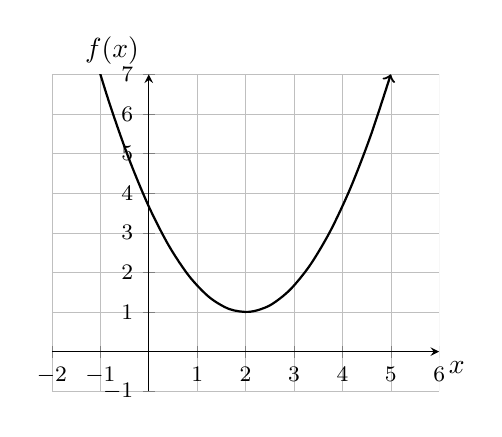
\begin{tikzpicture}
            \begin{axis}[
              DefaultPlotStyle,
              xmin = -2,
              xmax = 6,
              xtick={-6,-5,...,9},
              ymin = -1,
              ymax = 7,
              ytick={-10,-9,...,80},
            ]

              \addplot[
                thick,
                smooth,
                <->,
              ]
              { ((2*x^2 - (8 * x) + 8)/3) + 1 };
            \end{axis}
          \end{tikzpicture}
        \end{figure}
    \end{multicols}
\end{enumerate}

\end{document}

%%% Local Variables:
%%% mode: latex
%%% TeX-master: t
%%% End:
